\documentclass[
  digital,     %% The `digital` option enables the default options for the
               %% digital version of a document. Replace with `printed`
               %% to enable the default options for the printed version
               %% of a document.
%%  color,       %% Uncomment these lines (by removing the %% at the
%%               %% beginning) to use color in the printed version of your
%%               %% document
  oneside,     %% The `oneside` option enables one-sided typesetting,
               %% which is preferred if you are only going to submit a
               %% digital version of your thesis. Replace with `twoside`
               %% for double-sided typesetting if you are planning to
               %% also print your thesis. For double-sided typesetting,
               %% use at least 120 g/m² paper to prevent show-through.
  nosansbold,  %% The `nosansbold` option prevents the use of the
               %% sans-serif type face for bold text. Replace with
               %% `sansbold` to use sans-serif type face for bold text.
  nocolorbold, %% The `nocolorbold` option disables the usage of the
               %% blue color for bold text, instead using black. Replace
               %% with `colorbold` to use blue for bold text.
  lof,         %% The `lof` option prints the List of Figures. Replace
               %% with `nolof` to hide the List of Figures.
  lot,         %% The `lot` option prints the List of Tables. Replace
               %% with `nolot` to hide the List of Tables.
]{fithesis4}
%% The following section sets up the locales used in the thesis.
\usepackage[resetfonts]{cmap} %% We need to load the T2A font encoding
\usepackage[T1,T2A]{fontenc}  %% to use the Cyrillic fonts with Russian texts.
\usepackage[
  main=english, %% By using `czech` or `slovak` as the main locale
                %% instead of `english`, you can typeset the thesis
                %% in either Czech or Slovak, respectively.
  english, czech, slovak %% The additional keys allow
]{babel}        %% foreign texts to be typeset as follows:
%%
%%   \begin{otherlanguage}{german}  ... \end{otherlanguage}
%%   \begin{otherlanguage}{russian} ... \end{otherlanguage}
%%   \begin{otherlanguage}{czech}   ... \end{otherlanguage}
%%   \begin{otherlanguage}{slovak}  ... \end{otherlanguage}
%%
%% For non-Latin scripts, it may be necessary to load additional
%% fonts:
\usepackage{paratype}
\def\textrussian#1{{\usefont{T2A}{PTSerif-TLF}{m}{rm}#1}}
%%
%% The following section sets up the metadata of the thesis.
\thesissetup{
    date        = \the\year/\the\month/\the\day,
    university  = mu,
    faculty     = fi,
    type        = bc,
    department  = Department of Visual Computing,
    author      = Bruno Petrus,
    gender      = m,
    advisor     = {doc. RNDr. Martin Maška, Ph.D.},
    title       = {Segmentation of Membrane-Stained Cells in Image Data of Organoids},
    TeXtitle    = {Segmentation of Membrane-Stained Cells in Image Data of Organoids},
    keywords    = {keyword1, keyword2, ...},
    TeXkeywords = {keyword1, keyword2, \ldots},
    abstract    = {%
      This is the abstract of my thesis, which can

      span multiple paragraphs.
    },
    thanks      = {%
      These are the acknowledgements for my thesis, which can

      span multiple paragraphs.
    },
    bib         = bibliography.bib,
    %% Remove the following line to use the JVS 2018 faculty logo.
    facultyLogo = fithesis-fi,
}
\usepackage{makeidx}      %% The `makeidx` package contains
\makeindex                %% helper commands for index typesetting.
%% These additional packages are used within the document:
\usepackage{paralist} %% Compact list environments
\usepackage{amsmath}  %% Mathematics
\usepackage{amsthm}
\usepackage{amsfonts}
\usepackage{url}      %% Hyperlinks
\usepackage{markdown} %% Lightweight markup
\usepackage{listings} %% Source code highlighting
\lstset{
  basicstyle      = \ttfamily,
  identifierstyle = \color{black},
  keywordstyle    = \color{blue},
  keywordstyle    = {[2]\color{cyan}},
  keywordstyle    = {[3]\color{olive}},
  stringstyle     = \color{teal},
  commentstyle    = \itshape\color{magenta},
  breaklines      = true,
}
\usepackage{floatrow} %% Putting captions above tables
\floatsetup[table]{capposition=top}
\usepackage[babel]{csquotes} %% Context-sensitive quotation marks

%% Specify new commands
\newcommand*{\R}{\ensuremath{\mathbb{R}}}
\newcommand*{\Z}{\ensuremath{\mathbb{Z}}}

\begin{document}
%% The \chapter* command can be used to produce unnumbered chapters:
\chapter*{Introduction}
%% Unlike \chapter, \chapter* does not update the headings and does not
%% enter the chapter to the table of contents. I we want correct
%% headings and a table of contents entry, we must add them manually:
\markright{\textsc{Introduction}}
\addcontentsline{toc}{chapter}{Introduction}

Theses are rumoured to be \enquote{the capstones of education}, so
I decided to write one of my own. If all goes well, I will soon
have a diploma under my belt. Wish me luck!

\chapter{Theory}

\section{Digital Image}

Our eyesight is arguably one of our most useful sense for observing the world.
Researchers have developed many tools which helps us study the world. I will
begin by formalising the concept of an image, so that we can use mathematics
and computer science to talk about images.

Essentially we can think of an image as an n-dimensional function $f(x_1, x_2,
..., x_n)$, where $x_1, x_2, .. x_n$ are coordinates inside a spatial plane,
while the function value at those coordinates specify the magnitude or intensity
of the signal at that point. In most general term, we can think about images as
a functions of type $f:\R^n \rightarrow \R^m$, where $n$ indicates the number of
spatial dimensions and $m$ specifies the number of channels. For example when
we are talking about two-dimensional grayscale images, $m$ is equal to 1 and $n$ is
equal to 2, while a typical coloured photograph can have more than 3 channels.

In real life, we do not necessarily work with real valued spatial dimensions and
intensities, but only have a finite number of bits to work with. The process of
acquiring images in a finite grid and assigning a intensities from a finite
range is called sampling and quantization. In essence, we create a discretized
version of the original signal, which can be represented as an array of values.
This is what we call a digital image.

\subsection{Acquiring}

\subsection{Sampling}

\subsection{Noise}

Unfortunately when we rarely acquire a perfect image without any noise. Noise
can be thought of as an unwanted variations in image intensities which are not
present in the original signal. Noise in the signal may arise during multiple
steps of the process, for example it might a fault of an imperfect sensor which,
such as when we deal with charged-coupled device cameras. There a light input is
converted into an electric signal, but such sensors only have a limited quantum
efficiency and are greatly affected by the environmental factors such as the
temperature and light intensity. After the sensor a common source of noise is
the signal's transmission. It is greatly affected by disturbances in the used
channel, such as low energy due to distance during wireless transmission or
limited baud rate of WiFi or Bluetooth. While wireless interfaces have many
issues, a physical damage or the material's limitation may hinder the wired
alternative too.

\subsubsection{Typical noise in fluorescence microscopy.}

Generally each source of noise can behave differently and in process of restoring
images, the distribution and nature of noise is essential to know. According to
\parencite{hamamatsu_ccd} there are three main sources of noise when using CCD
sensors and those are:
\begin{compactenum}
\item Photon noise
\item Dark noise
\item Read noise
\end{compactenum}

TODO

\section{Edge finding}
TODO

\section{Thresholding}
TODO

\section{Mathematical morphology}

Mathematical morphology is a tool used to extract various interesting features
from images. The tasks include edge detecting algorithms, thinning, prunning,
convex hulls, and filtering just to name a few. In the most simple terms,
mathematical morphology works on images using what we call structural elements.
Those can take many form, but their shape varies based on the task we are trying
to achieve. In this thesis we will mainly focus on using mathematical morphology
to pre and post process image data generated by other image processing methods.
We will start by looking at some basic operations on binary image. Note that
this area is very large and I will cover only parts which are useful later in my
prototype.

In this branch of image processing we look at the images through set theory
instead of looking at images as discrete-valued functions. In this context, an
image is a subset of 2-D integer space $\Z^2$, but it can easily be generalized
to more dimensions. Each element of this subset $(x, y)$ represents a present
pixel at those coordinates in the image. In other words, if we look at an image
as an array of rectangular shape, then each foreground pixel's coordinates will
be included inside the final set.

\subsection{Preliminary}
Before we look at the main two operations - erosion and dilation, we have to
define two not so common operations on sets which are heavily used in
mathematical morphology.

During the following definition we need to be able to talk about how to create a
reflection of the image around origin as is shown on the figure
\ref{fig:morp_refl}. It is defined as: 
$$\hat{B} = \{w | w=-b \text{ , for } b \in B\}$$
\begin{figure}
    \begin{center}
        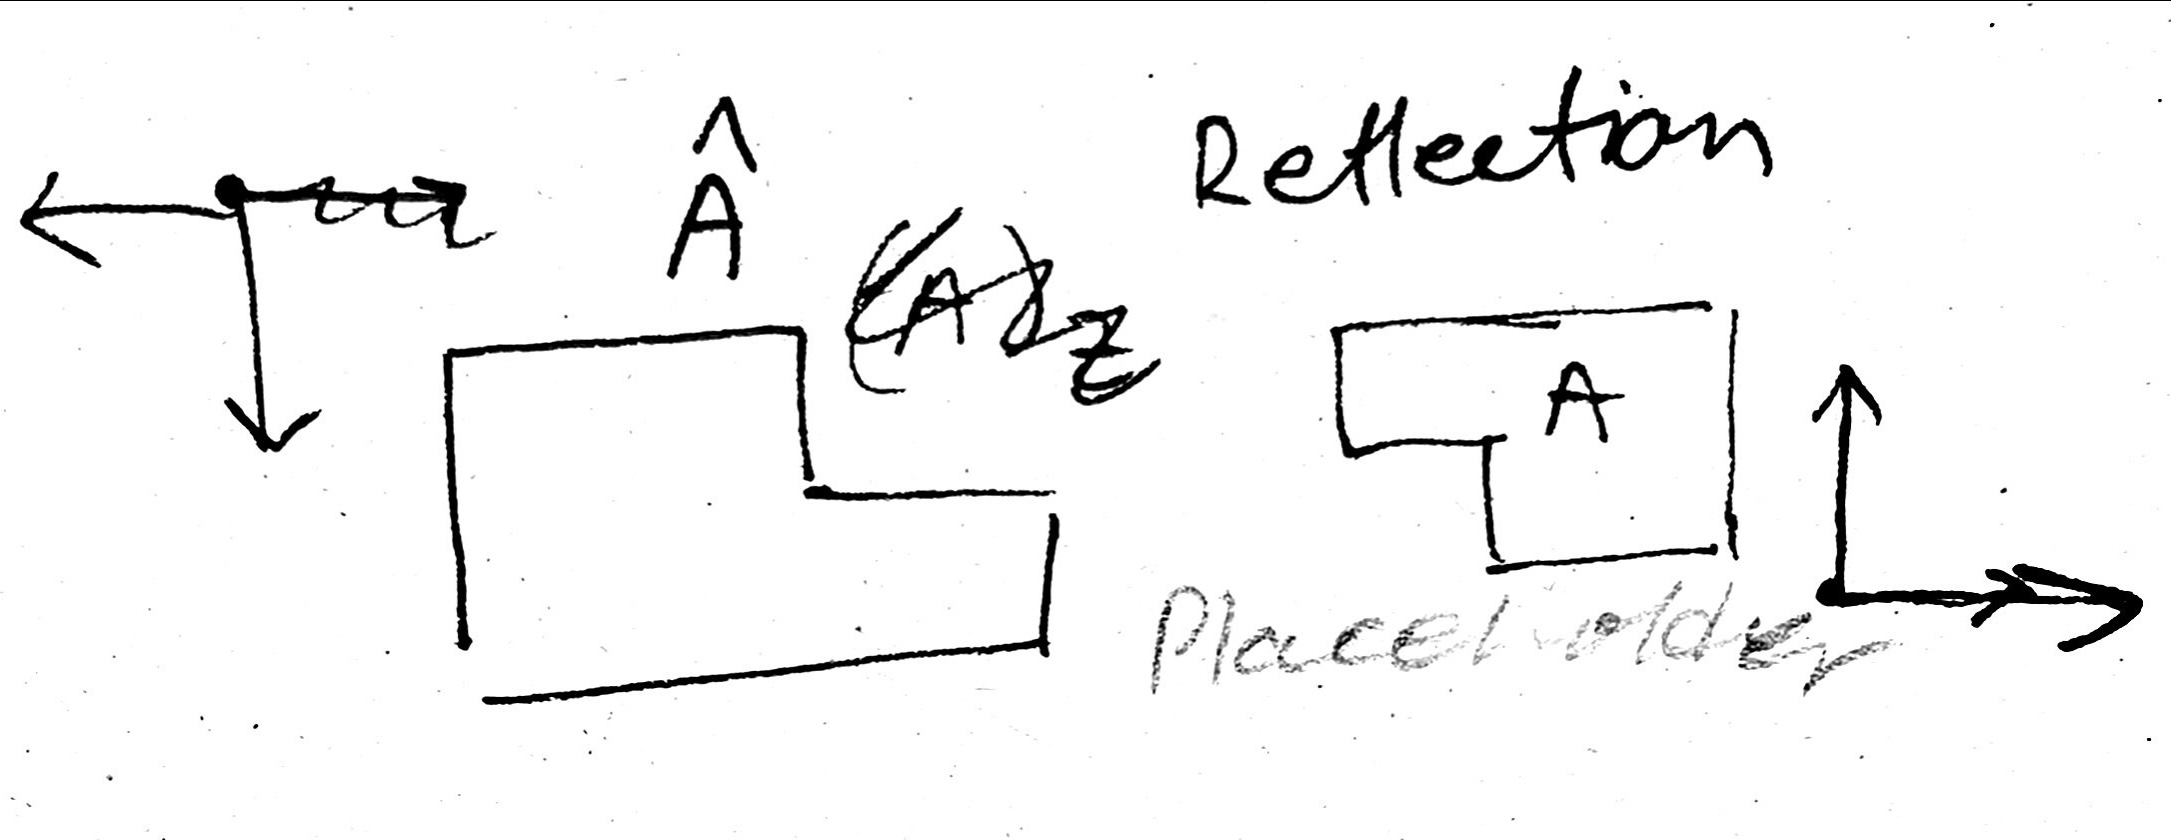
\includegraphics[width=6.3cm]{resources/morph_reflection.jpg}
    \end{center}
    \caption{Morphological reflection} % todo: replace
    \label{fig:morp_refl}
\end{figure}

While manipulating images we commonly have to move parts of the image around. We
define a similar operation on sets, called translation. The formal definition of
moving a set $A$ by some translation vector $z$ is:
$$(A)_z = \{c | c = a + z\text{ , for } a \in A\}$$
The operation is illustrated on figure \ref{fig:morph_translation} where the set
$B$ is moved downwards by a vector $z$.
\begin{figure}
    \begin{center}
        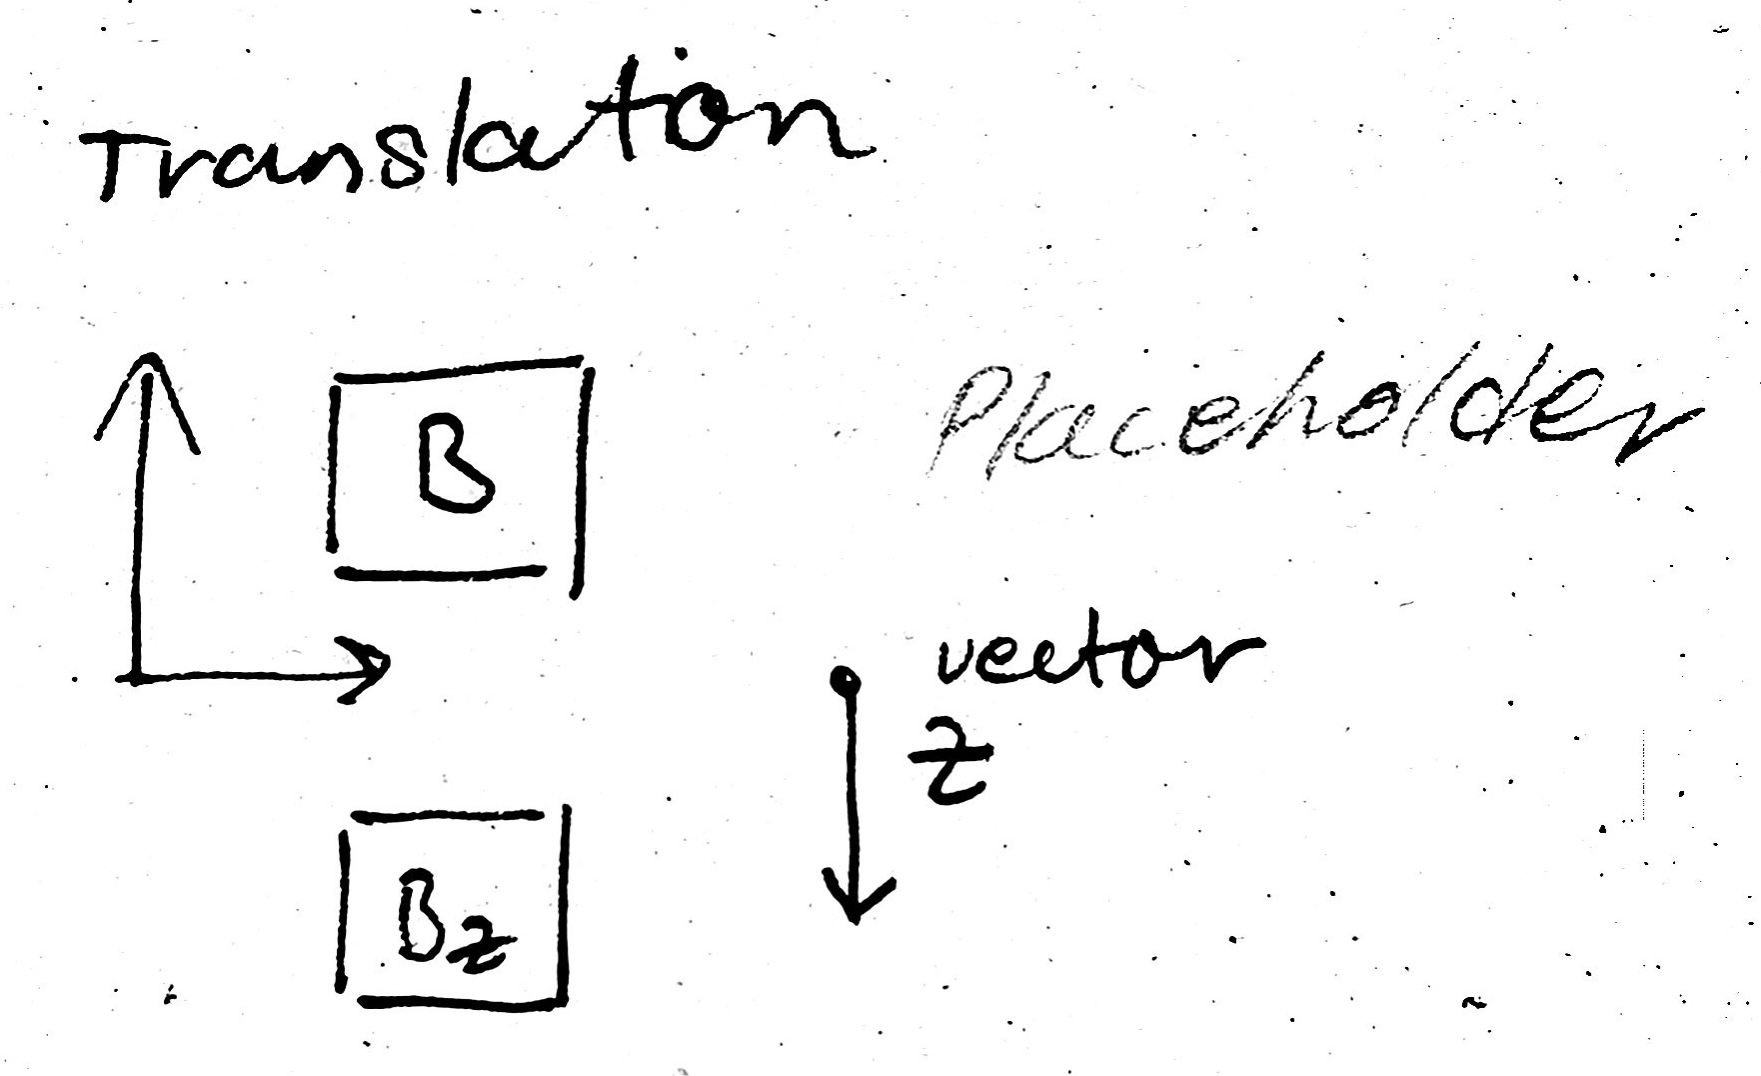
\includegraphics[width=6.3cm]{resources/morph_translation.jpg}
    \end{center}
    \caption{Morphological translation} % todo: Replace
    \label{fig:morph_translation}
\end{figure}

\subsection{Dilation and Erosion}
Now we are ready to properly define two fundamental operations in the field of
mathematical morphology, upon which many other operations are built. Both of
these operations include a structural element. A structural element is again a
set, but it can be used to describe how far or how much the dilation and erosion
operations can go.

\subsubsection{Dilation}
First let's look at the dilation operation. Intuitively we can think about this
operator as a way to dilate the set into bigger space. Formally it is defined as
$$A \oplus B = \{z | (\hat{B}_z) \cap A \neq \emptyset\}$$
where $A$ and $B$ are both sets in $\Z^2$. 

An example of dilation can be seen on the figure
\ref{fig:morph_dilation}. There we have two examples. In the first row, we have
a square image with side length $d$ and a structuring element, whose side length
is a fourth of the original. If we apply the dilation operation on these two
images we get the one on the right. You can image taking the smaller square and
gliding it over the bigger one. If there is an overlap, we can add the centre of
the structural element to the result. 

Closer to the mathematical definition, we
are translating the structural element $B$ using all possible translation
vectors $z$ and if there is an overlap, we add the centre of the element to the
result.

This operation can be used to for example join disconnected segments in an
image by choosing a large enough structural element. Its size will depend on the
particular example and does not have to necessarily be of regular size.

\begin{figure}
    \begin{center}
        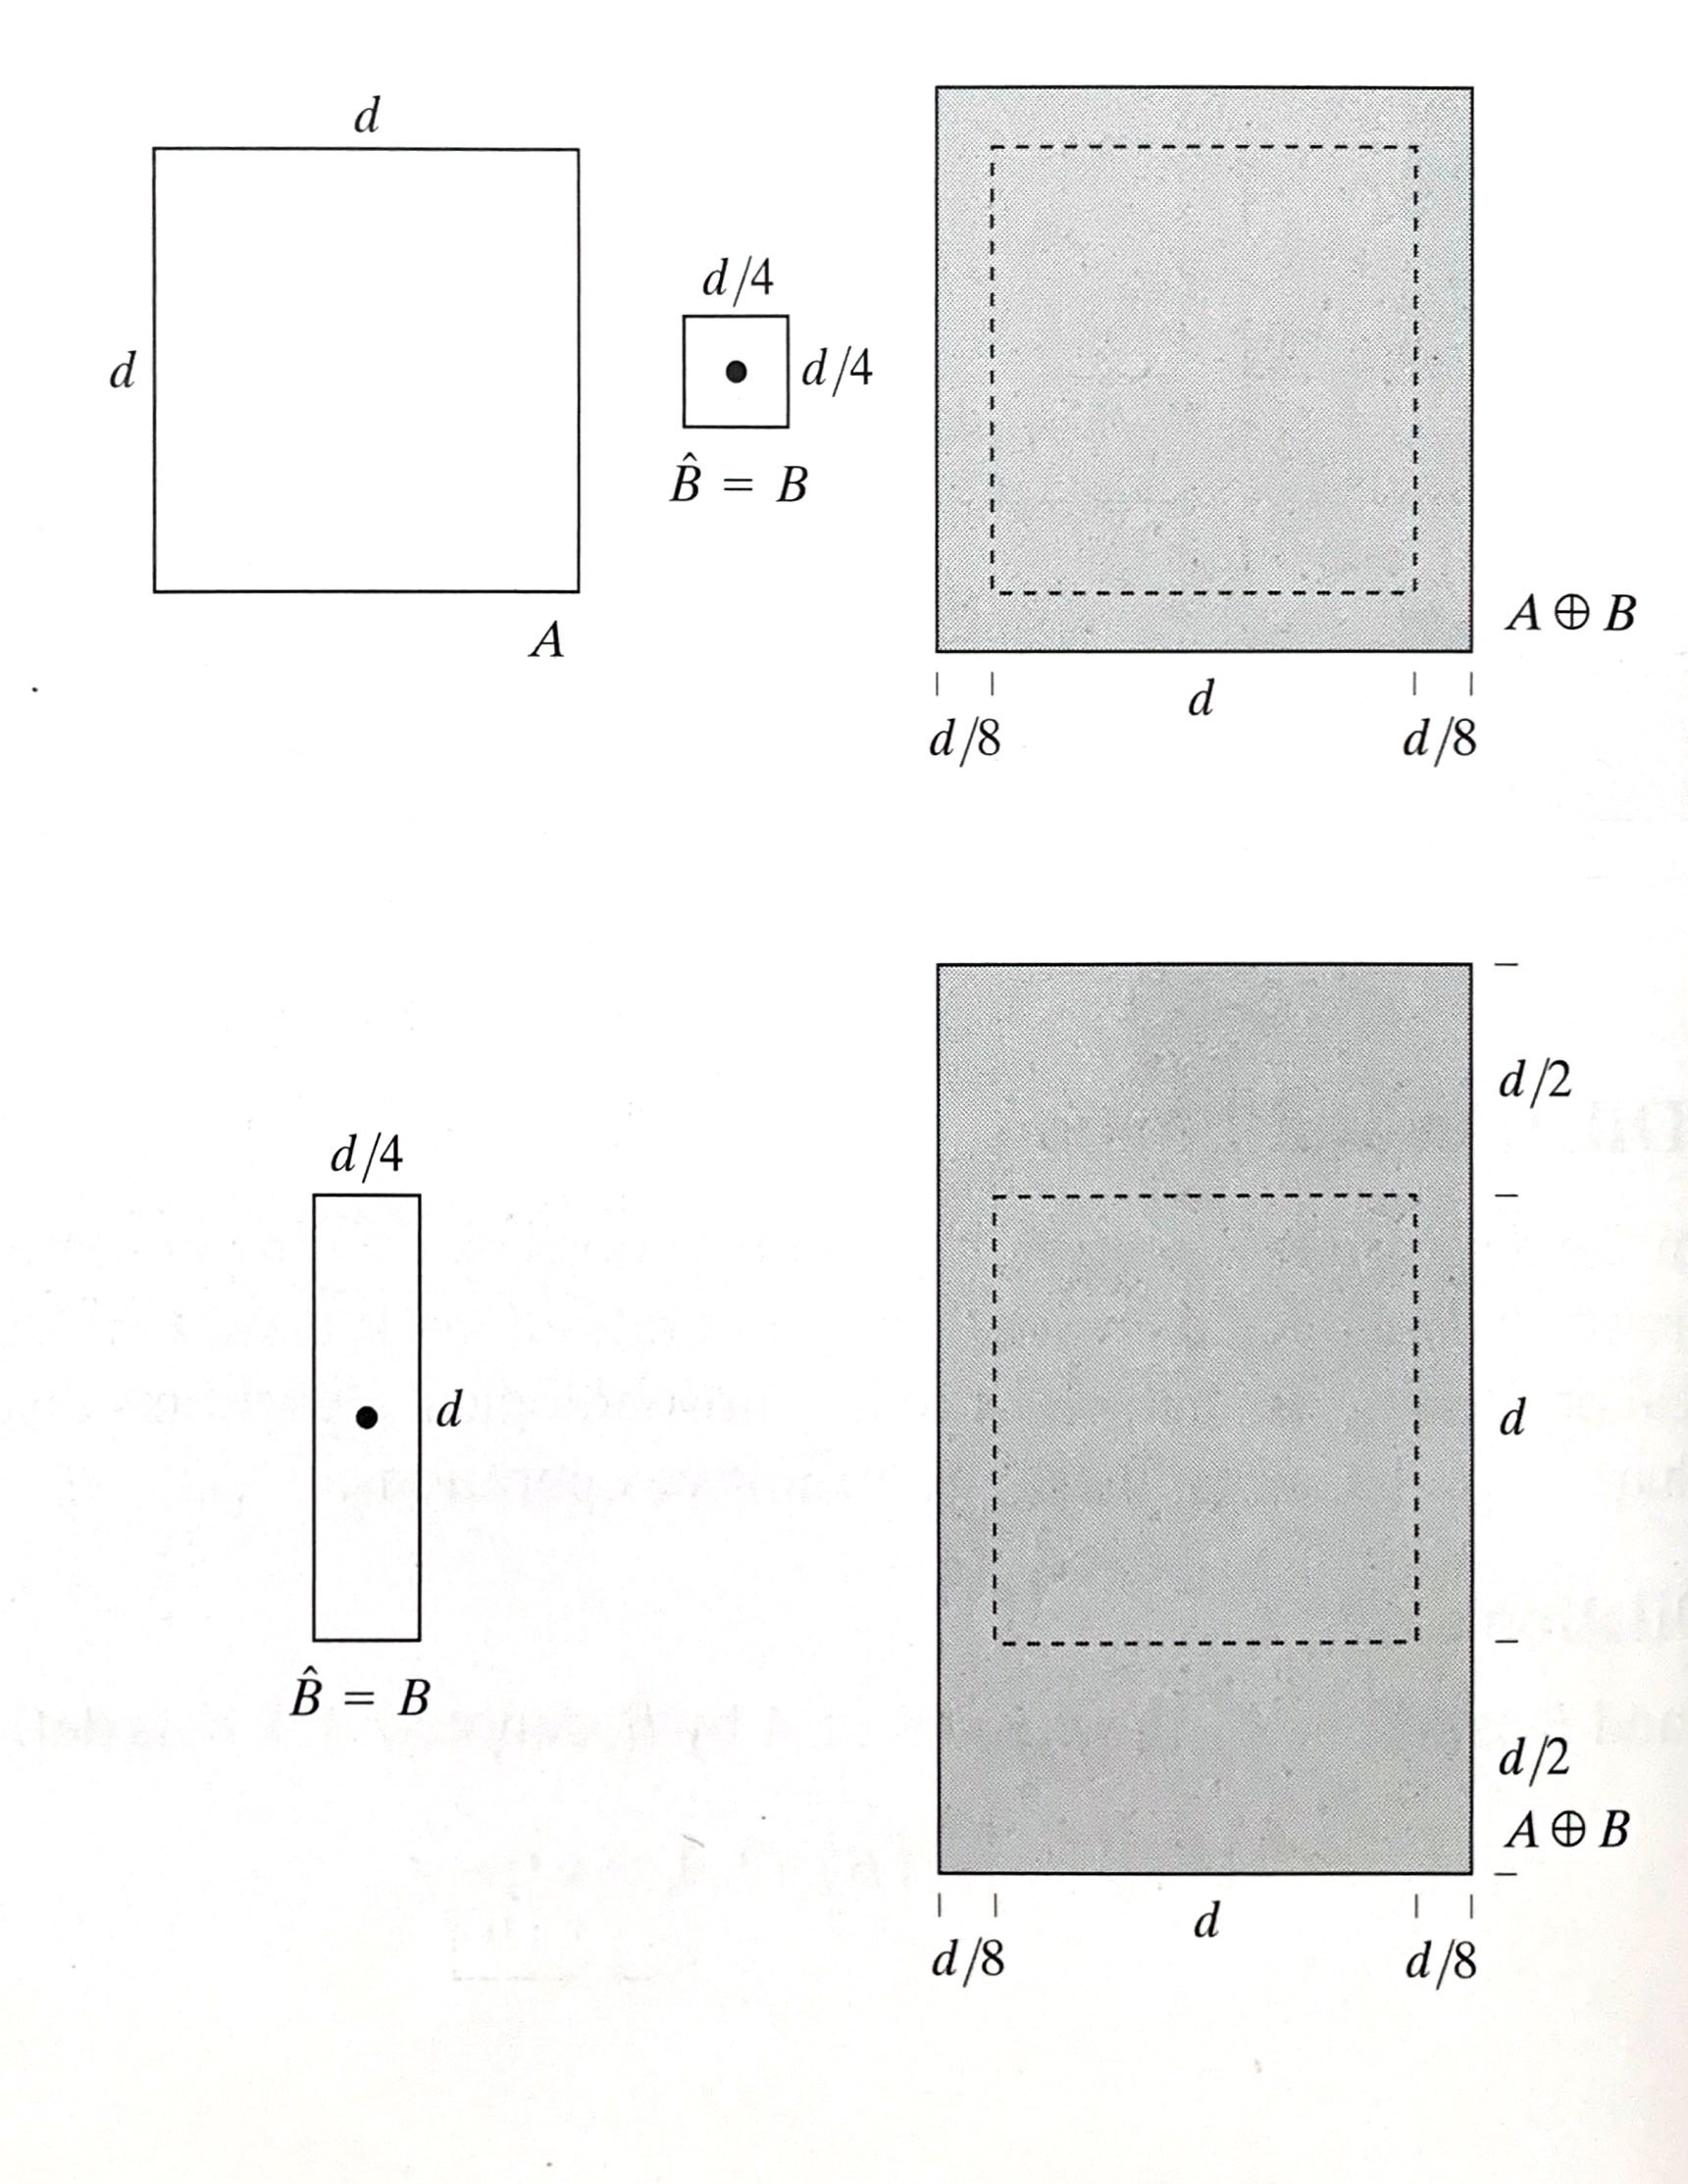
\includegraphics[width=6.3cm]{resources/morph_dilation.jpg}
    \end{center}
    \caption{Morphological dilation (Gonzalez 2002)} % todo: Replace
    \label{fig:morph_dilation}
\end{figure}

\subsubsection{Erosion}

Next essential operation is erosion. As the name suggest we use it to erode
parts of the image, which we consider unnecessary. An erosion $A \ominus B$ of
two sets $A$ and $B$, both part of $\Z^2$ space, is defined as: 
$$A \ominus B = \{z | (B)_z \subseteq A\}$$

Again $A$ can be though as an image while $B$ can be looked at as a structural
element. In contrast to dilation operation we are now looking if the whole
structural element fits inside $A$ as can be seen in figure
\ref{fig:morph_erosion}. There a smaller structural element is used to cut away
parts of the bigger square.

As opposed to the dilation, we can use erosion to divide lightly connected
segments, and to erase noise and other unwanted disturbances in an image.

While mathematical morphology is a massive topic of interest to many
researchers, here I will only use the aforementioned operations. They can be
further used to define more operations such as binary opening and binary closing
and can be expanded to include grayscale images, however I will not be using or covering
them in my thesis.

\begin{figure}
    \begin{center}
        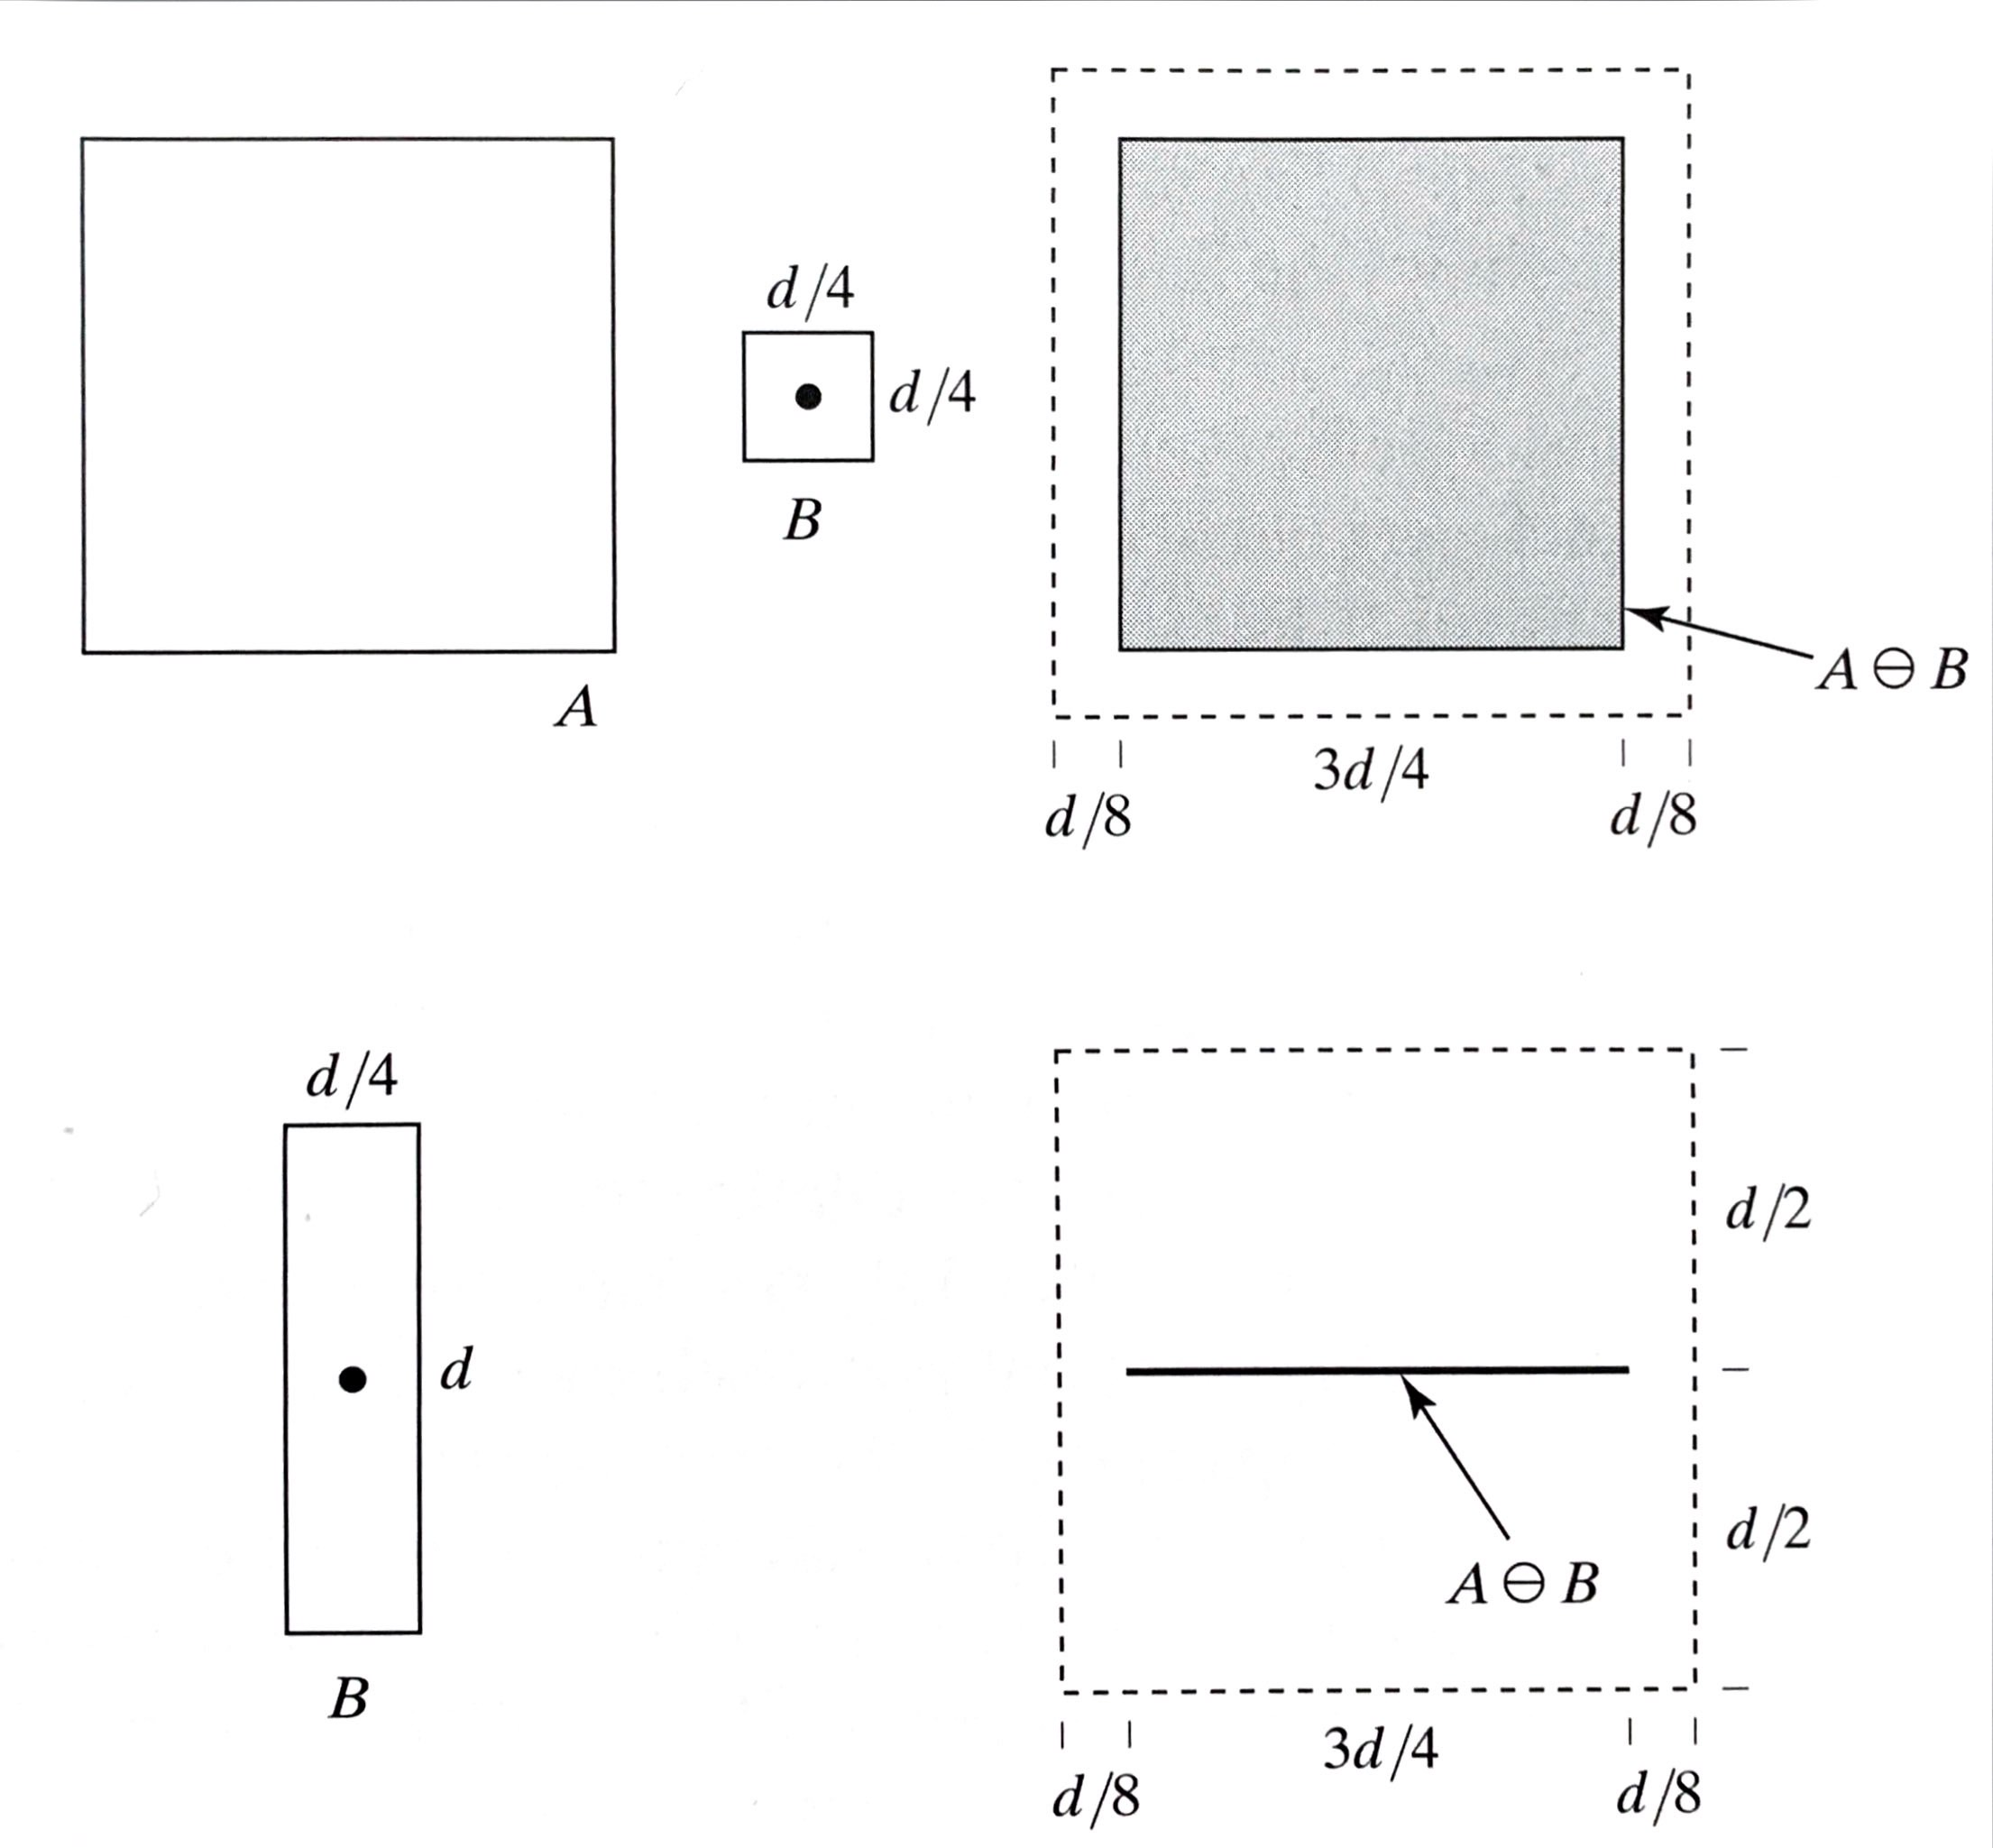
\includegraphics[width=6.3cm]{resources/morph_erosion.jpg}
    \end{center}
    \caption{Morphological erosion (Gonzalez 2002)} % todo: Replace
    \label{fig:morph_erosion}
\end{figure}

\section{Segmentation}



\end{document}
